\documentclass[journal]{IEEEtran}

% ================================================
% Core Packages
% ================================================
\usepackage[utf8]{inputenc}
\usepackage[T1]{fontenc}
\usepackage{hyperref}
\usepackage{url}
\usepackage{booktabs}
\usepackage{amsfonts}
\usepackage{amsmath}
\usepackage{amssymb}
\usepackage{mathtools}
\usepackage{graphicx}
\usepackage{xcolor}
\usepackage{microtype}
\usepackage{comment}
\usepackage{subcaption}      % for subfigures
\usepackage{multirow}
\usepackage{tabularx}
\usepackage{array}
\usepackage{colortbl}

% Algorithm packages
\usepackage{algorithm}
\usepackage{algorithmic}

% Natbib for IEEE numerical citations [1], [2-5], etc.
\usepackage[numbers, square, sort&compress]{natbib}

% ================================================
% Macros
% ================================================
\newcommand{\agentforge}{\textsc{AgentForge}}
\newcommand{\swebench}{\textsc{SWE-bench}}
\newcommand{\eg}{\textit{e.g.,}\ }
\newcommand{\ie}{\textit{i.e.,}\ }
\newcommand{\etal}{\textit{et al.}}

% ================================================
% Title and Authors (IEEE style)
% ================================================
\title{AgentForge: Execution-Grounded Multi-Agent LLM Framework for Autonomous Software Engineering}

\author{
    Rajesh~Kumar, %
    \thanks{R. Kumar with International Research Center for Complexity Sciences, Hangzhou International Innovation Institute, Beihang University, Hangzhou, 311115, China(e-mail: rajakumarlohano@gmail.com}%
    Waqar~Ali, %
    \thanks{W. Ali is with the Department of Computer Science, College of Science, Mathematics and Technology, Wenzhou-Kean University, Wenzhou 325060, China (e-mail: waqar.uestc@yahoo.com).}%
    %
    Junaid~Ahmed, %
     \thanks{ J. Ahmed is with Computer Systems Engineering Department, Sukkur IBA University, Sindh , Pakistan (e-mail: j.bhatti@iba-suk.edu.pk) }%
     %
    Najma~Imtiaz~Ali, %
     \thanks{N.Imtiaz is with Fakulti Teknologi Maklumat dan Komunikasi, Universiti Teknikal Malaysia Melaka, Melaka 76100, Malaysia (e-mail:  najma@utem.edu.my).}%
     %
    Shaban~Usman, %
     \thanks{S. Usman is with Yibin Park of University of Electronic Science and Technology of China, Yibin 644000, China (e-mail:  shabanusman@yahoo.com).}%

}


% ================================================
% Document Start
% ================================================
\begin{document}

% Title + Authors
\maketitle

% ================================================
% Abstract
% ================================================
\begin{abstract}
Large language models generate plausible code but cannot verify correctness. Existing multi-agent systems simulate execution or leave verification optional. We introduce execution-grounded verification as a first-class principle: every code change must survive sandboxed execution before propagation. We instantiate this principle in \agentforge{}, a multi-agent framework where Planner, Coder, Tester, Debugger, and Critic agents coordinate through shared memory and a mandatory Docker sandbox. We formalize software engineering with LLMs as an iterative decision process over repository states, where execution feedback provides a stronger supervision signal than next-token likelihood. \agentforge{} achieves 40.0\% resolution on \swebench{} Lite, outperforming single-agent baselines by 26--28 points. Ablations confirm that execution feedback and role decomposition each independently drive performance. The framework is open-source at \url{https://github.com/raja21068/AutoCodeAI}.
\end{abstract}

% Optional: IEEE Keywords (strongly recommended)
\begin{IEEEkeywords}
Multi-agent systems, Large language models, Automated program repair, Execution verification, Software engineering, SWE-bench
\end{IEEEkeywords}
% ============================================================
%  Section 1: Introduction
% ============================================================

\section{Introduction}
\label{sec:intro}

Large language models (LLMs) perform well on code generation but remain unreliable for real-world software engineering. Practical tasks require reasoning over existing codebases, executing programs, and iteratively refining solutions under test feedback. Most current systems treat code generation as a single-step prediction problem, mapping a natural language description to a code completion~\cite{brown2020language}. This approach fails on tasks that require multi-file reasoning, test generation, and regression avoidance~\cite{chen2021codex}.


Recent work addresses these limitations with multi-agent systems that decompose development into roles such as planning, coding, testing, and reviewing. Such approaches boost the benchmark SWE-bench by means of a structural interaction among agents~\cite{trae2025}. Nevertheless, there is a major drawback to these approaches: none of the proposed frameworks provide guaranteed grounded execution, as all of them guess execution results or work under permissive conditions.


This limitation is critical. Bug fixing requires a feedback loop plan, implement, execute, test, and revise driven by real execution signals. Without grounded feedback, models cannot reliably verify correctness or detect regressions. Simulated execution introduces systematic errors that propagate through the pipeline.


We introduce \textbf{AgentForge}, a multi-agent framework that enforces verified execution for autonomous software engineering. AgentForge decomposes bug fixing into five specialized agents: \textit{Planner}, \textit{Coder}, \textit{Tester}, \textit{Debugger}, and \textit{Critic}. The Planner generates a structured execution plan. The Coder produces minimal patches using unified diffs. The Tester synthesizes executable test cases. The Debugger iteratively repairs failures using execution feedback. The Critic validates the final result.

AgentForge grounds all decisions in two retrieval sources: (i) episodic memory of previously solved tasks and (ii) a live repository index of the current codebase. The system executes every generated patch inside a resource-constrained, network-isolated Docker sandbox. This design provides non-simulated execution feedback and enables a closed-loop Tester--Debugger cycle for iterative repair.

% RC1: Clarified novelty claim -- prior work (OpenHands, SWE-agent) offers sandboxing
% as an optional feature or final validation step; AgentForge mandates it after every
% single code change as a structural orchestration requirement, not a flag.
Table~\ref{tab:frameworks_axes} situates AgentForge among existing systems. Unlike OpenHands and SWE-agent, which provide sandboxing as an optional tool or final validation step, AgentForge requires verified execution after every patch. The Tester and Debugger agents cannot proceed unless sandboxed outcomes are obtained, creating a closed-loop execution guarantee. Prior frameworks introduce role decomposition, knowledge graphs, or test-time scaling~\cite{khanzadeh2025agentmesh,tao2024magis,sgagent2026,trae2025}. Other methods have been proposed for self-evolution and competition~\cite{ecoevolve2026,swedebate2026}. None incorporate sandboxing during mandatory execution alongside dual recall with the entire five-agent architecture. AgentForge consolidates all these elements under one execution.


\begin{comment}
\begin{table}[t]
\centering
\caption{Comparison of representative multi-agent frameworks. AgentForge uniquely
         combines mandatory sandboxed execution, dual retrieval, and an independent Critic agent.}
\label{tab:comparison}
\small
\setlength{\tabcolsep}{5pt}
\renewcommand{\arraystretch}{1.25}
\newcolumntype{Y}{>{\centering\arraybackslash}p{2.0cm}}

\begin{tabular}{@{} l p{2.6cm} p{2.1cm} p{2.1cm} p{2.1cm} p{2.3cm} @{}}
\toprule
\textbf{Feature}
  & \cellcolor{blue!8}\textbf{AgentForge (ours)}
  & \textbf{AgentMesh}~\cite{khanzadeh2025agentmesh}
  & \textbf{MAGIS}~\cite{tao2024magis}
  & \textbf{SGAgent}~\cite{sgagent2026}
  & \textbf{Trae Agent}~\cite{trae2025} \\
\midrule

\multicolumn{6}{@{}l}{\textit{\small\color{gray} Architecture}} \\[1pt]

Agent roles
  & \cellcolor{blue!8}Planner, Coder, Tester, Debugger, \textbf{Critic}
  & Planner, Coder, Debugger, Reviewer
  & Manager, Custodian, Developer, QA
  & Localizer, Suggester, Fixer
  & Generator, Pruner, Selector \\

Independent critic
  & \cellcolor{blue!8}\textbf{Yes} --- dedicated agent
  & Yes --- Reviewer
  & Implied (QA)
  & No
  & No \\[4pt]

\multicolumn{6}{@{}l}{\textit{\small\color{gray} Execution}} \\[1pt]

Verified execution
  & \cellcolor{blue!8}\textbf{Mandatory} Docker sandbox
  & --
  & --
  & --
  & Supported \\

Iterative debug loop
  & \cellcolor{blue!8}\textbf{Yes}, configurable retries
  & Yes
  & Implied (QA)
  & Yes
  & Yes (test-time scaling) \\[4pt]

\multicolumn{6}{@{}l}{\textit{\small\color{gray} Memory}} \\[1pt]

Memory / retrieval
  & \cellcolor{blue!8}\textbf{Dual}: episodic + repo index
  & --
  & --
  & Knowledge graph
  & -- \\[4pt]

\multicolumn{6}{@{}l}{\textit{\small\color{gray} Evaluation (SWE-bench)}} \\[1pt]

Reported metric
  & \cellcolor{blue!8}\textbf{40.0\%} resolution
  & Not evaluated
  & 13.94\% resolution
  & 51.3\% repair acc.
  & 75.20\% Pass@1 \\

\bottomrule
\end{tabular}
\end{table}
\end{comment}

% RC1: Table I updated to clarify that SWE-agent and OpenHands offer sandboxing as
% optional, whereas AgentForge mandates it structurally after every patch.
\begin{table*}[t]
\centering
\caption{Positioning Multi-Agent Frameworks Along Three Axes. SWE-agent and OpenHands
         offer sandboxing as an optional tool or final validation step; AgentForge mandates
         it after every patch as a structural orchestration requirement.}
\label{tab:frameworks_axes}
\small
\setlength{\tabcolsep}{5pt}
\renewcommand{\arraystretch}{1.25}

\begin{tabular}{@{} l p{3.5cm} p{3.5cm} p{3.5cm} @{}}
\toprule
\textbf{Framework}
  & \textbf{Execution Feedback}
  & \textbf{Role Decomposition}
  & \textbf{Memory/Retrieval} \\
\midrule

\textbf{AgentForge}
  & \textbf{Mandatory} sandbox (every patch)
  & 5 roles (plan, code, test, debug, critic)
  & Dual (episodic + repo) \\

\textbf{SWE-agent}
  & Shell/ACI (\textit{optional})
  & Single agent
  & None \\

\textbf{OpenHands}
  & Sandbox (\textit{optional})
  & Single agent
  & None \\

\textbf{Trae Agent}
  & Test-time scaling
  & 3 roles (gen, prune, select)
  & None \\

\textbf{MAGIS}
  & Implied
  & 4 roles (mgr, custodian, dev, qa)
  & None \\

\textbf{AgentMesh}
  & None
  & 3 roles (plan, debug, review)
  & None \\

\textbf{Reflexion}
  & Simulated
  & Single + self-reflection
  & Episodic memory \\

\bottomrule
\end{tabular}
\end{table*}

\textbf{Contributions.}
\begin{itemize}
    \item We formalize LLM-based software engineering as an \textit{execution-grounded iterative refinement problem}, where correctness is defined by external program execution rather than model-internal likelihood signals.

    % RC2: Removed claim that we learn a policy. MDP is used for analytical/descriptive
    % purposes only; policy optimization is left as future work.
    \item We model this process as a finite-horizon Markov decision process (MDP) for analytical purposes. The MDP describes feedback, credit assignment, and error propagation in the environment; our implementation follows a fixed orchestration and does not perform policy optimization.

    \item We identify two key properties: (i) execution feedback provides a stronger supervision signal for functional correctness than next-token likelihood, and (ii) decomposing generation, testing, and debugging reduces error accumulation compared to monolithic self-repair.

    \item We instantiate these principles in \agentforge{}, a five-agent framework with structured orchestration, dual retrieval (episodic memory and repository index), and mandatory Docker-based execution.

\end{itemize}

\textbf{Novelty summary.} AgentForge is the first framework to mandate sandboxed verification for every code change, providing ground-truth execution feedback after each individual patch rather than as a final validation step. It integrates five specialized agents (Planner, Coder, Tester, Debugger, Critic) with a dual-memory system (episodic memory + live repository index) -- a combination absent from AgentMesh, MAGIS, SGAgent, and Trae Agent.

\textbf{Implications.} Our results indicate that verified execution feedback and structured pipeline design matter more than raw model scale for real-world software engineering. AgentForge provides an open-source baseline for future research in this direction.

The remainder of this paper is organized as follows. Section~\ref{sec:related} surveys related work. Section~\ref{sec:method} details the AgentForge architecture. Section~\ref{sec:experiments} describes the experimental setup and baselines. Section~\ref{sec:results} presents main results and ablations. Section~\ref{sec:conclusion} discusses limitations and future directions.

% ============================================================
%  Section 2: Related Work
% ============================================================
\begin{figure*}[ht]
    \centering
    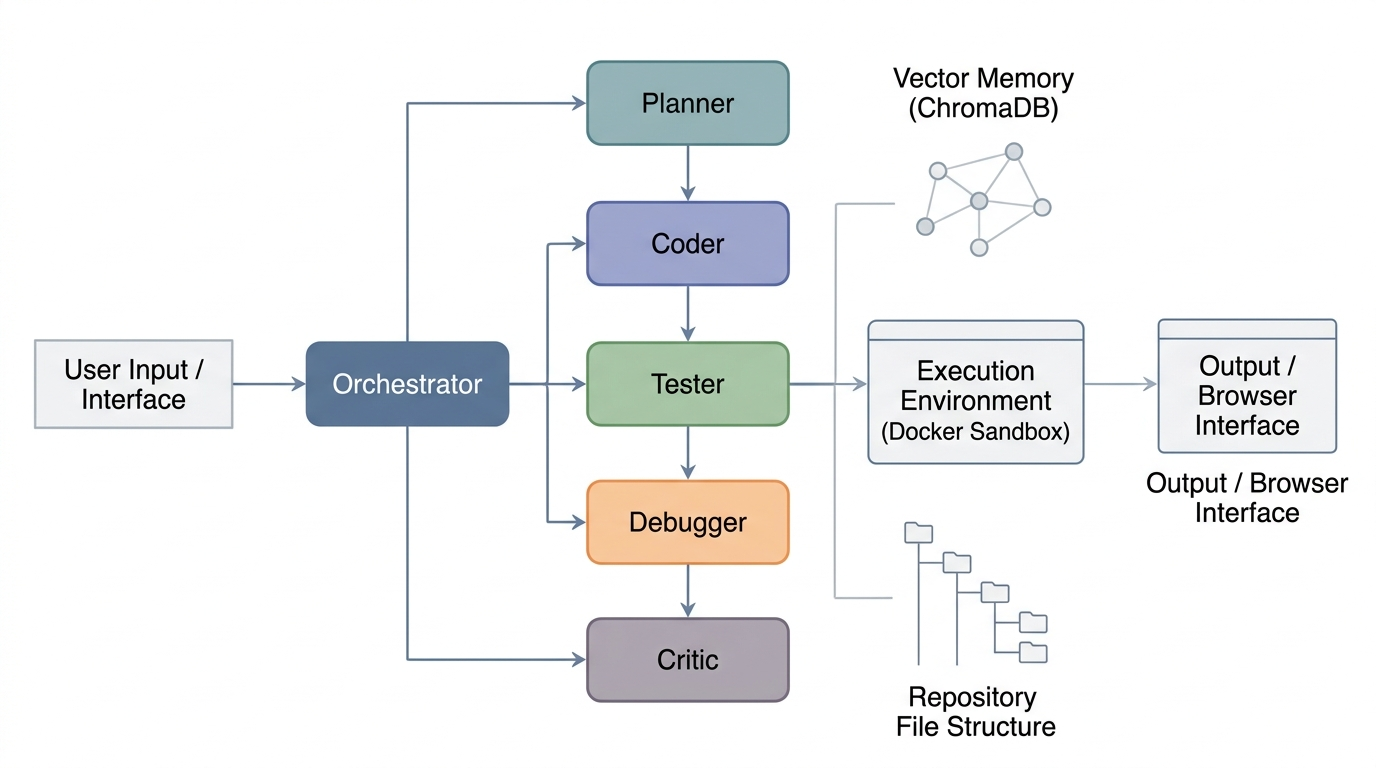
\includegraphics[width=\linewidth]{Figure1.png}
    \caption{Overview of the AgentForge multi-agent coding framework, illustrating the sequential handover between specialized agents and the shared Vector Memory.}
    \label{fig:overview}
\end{figure*}

\section{Related Work}
\label{sec:related}

\subsection{LLM-Based Code Generation}

Generation of neural codes started with the training of sequence-to-sequence models using paired text-code datasets~\cite{iyer2016summarizing,yin2017syntactic}. Training with large-scale pre-training on combined datasets altered this trend. Codex~\cite{chen2021codex} showed how a GPT architecture trained on GitHub could solve a significant portion of programming problems in one attempt. Further improvements were made by AlphaCode~\cite{li2022alphacode}, StarCoder~\cite{li2023starcoder}, and CodeLlama~\cite{roziere2023codellama} by leveraging scale, tokenizer, and optimization of the objective function suitable for coding editing. These models work under the framework of generating programs in a one-shot manner, without any mechanism for feedback-driven verification and correction based on failure conditions. This shortcoming justifies the need for a structured approach to solving programming problems. AgentForge uses a loop-based framework in which the code is tested and revised with real feedback.

\subsection{Program Repair and Iterative Refinement}

Automated program repair (APR) came before neural methods~\cite{le2012genprog}. Modern APR systems employ LLMs to suggest patches based on failing tests and localization signals~\cite{xia2022less,jin2023inferfix,fan2023automated}. These methods assume that the locations of the faults and the test suites are already known. Several recent papers make the feedback mechanism more effective. TraceRepair~\cite{tracerepair2026} constrains patches based on execution traces. DynaFix~\cite{dynafix2025} adds call stacks and runtime states to feedback. Interactive debugging is enabled in InspectCoder~\cite{inspectcoder2025} thanks to user control of the system. RGD~\cite{rgd2024} decomposes code fixing into three components: Guide, Debug, and Feedback.

Self-repair~\cite{olausson2023selfrepair} and self-debugging~\cite{chen2023teaching} have been used to modify the outputs of a single model with help from error messages. Both approaches merge generation and code fixing into one unified policy. AgentForge separates these tasks into individual agents, each having its own goals and interfaces. This leads to measurable improvements in our ablation study (Section~\ref{sec:ablation}).

\subsection{Agentic and Tool-Using LLM Systems}

ReAct~\cite{yao2023react} interleaves reasoning traces with tool calls, enabling closed-loop interaction with external environments. Reflexion~\cite{shinn2023reflexion} augments this loop with episodic memory via self-generated feedback. Both frameworks rely on a single model to plan, act, and evaluate. AgentForge distributes these roles across specialized agents. Each agent operates under a fixed contract and prompt. This design reduces per-call complexity and enforces structured intermediate representations. Toolformer~\cite{schick2023toolformer} learns tool invocation through self-supervision. It removes explicit prompting but requires fine-tuning and offers limited control over execution structure. AgentForge enforces explicit sequencing of planning, coding, testing, and debugging.

\subsection{Multi-Agent LLM Frameworks}

Multi-agent systems decompose complex tasks into role-specific components. MetaGPT~\cite{hong2023metagpt} encodes software roles through structured documents. ChatDev~\cite{qian2023chatdev} uses conversational agents to produce complete projects. AutoGen~\cite{wu2023autogen} provides a general interface for agent interaction and tool use. Recent systems introduce adaptive and competitive coordination. SEMAG~\cite{semag2026} evolves agent behavior with task difficulty. Eco-Evolve~\cite{ecoevolve2026} uses dynamic topologies and hindsight replay. SWE-Debate~\cite{swedebate2026} applies multi-round debate with search-based patch generation. These systems improve coordination but do not enforce execution-grounded validation at every step. AgentForge targets repository-level bug fixing and requires sandboxed execution for each candidate patch. It combines role specialization with mandatory verification and repository-grounded context.

\subsection{Autonomous Software Engineering Agents}

SWE-agent~\cite{yang2024sweagent} introduces an agent--computer interface that exposes shell, editor, and search tools to a single model. Devin~\cite{cognition2024devin} demonstrates end-to-end autonomous engineering, though its architecture remains undisclosed. OpenHands~\cite{wang2024openhands} provides an open-source platform with sandboxed execution. Trae Agent~\cite{trae2025} applies test-time scaling via generation, pruning, and selection. MAGIS~\cite{tao2024magis} decomposes issue resolution into Manager, Custodian, Developer, and QA roles.
AgentForge adopts explicit multi-agent decomposition with five specialized roles. Each agent produces a constrained artifact: plan, diff, tests, repairs, or review. This design enables controlled execution, modular analysis, and interpretable ablations.

\subsection{Benchmarks for Software Engineering}

Tasks such as HumanEval~\cite{chen2021codex} and MBPP~\cite{austin2021program} measure code generation from documentation strings. They focus only on generation, not taking repository context into account. SWE-bench~\cite{jimenez2024swebench} adds realistic GitHub tickets combined with test cases. SWE-bench Lite reduces cost while preserving diversity. SWE-bench Verified provides human-validated instances. Defects4J~\cite{defects4j} remains a standard benchmark for Java repair.

We evaluate on SWE-bench Lite following recent work~\cite{yang2024sweagent,wang2024openhands,zhang2024autocoderover}. This setting captures multi-file reasoning, environment interaction, and regression constraints.

\subsection{Memory and Retrieval in LLM Systems}

Retrieval-augmented generation (RAG) conditions models on external context to improve accuracy~\cite{lewis2020rag}. In code, repository-level retrieval supplies relevant files and functions for completion~\cite{zhang2023repocoder,shrivastava2023repofusion}.

AgentForge implements dual retrieval. It maintains episodic memory of past tasks and a live repository index. Both reside in a shared ChromaDB vector store and use cosine similarity over OpenAI text embeddings. Episodic memory enables cross-task transfer. Repository indexing ensures intra-task grounding. This unified retrieval design supports consistent context across all agents.

% ============================================================
%  Section 3: Method
% ============================================================

\section{Method}
\label{sec:method}

We present \textbf{AgentForge}, a multi-agent framework for autonomous software engineering. Given a natural language task $\mathcal{T}$ and an optional set of context files $\mathcal{F} = \{f_1, \dots, f_n\}$, AgentForge produces verified, executable code $\hat{c}$ by routing the task through a structured pipeline of five specialized agents, each responsible for a single subtask. Figure~\ref{fig:overview} shows the full system.




\subsection{Analytical Model of Execution-Grounded Refinement}
\label{sec:formal}

% RC2 (revised): MDP is descriptive only -- captures feedback structure and error
% propagation. Implementation follows fixed orchestration (Algorithm 1); no policy
% learning. Full MDP equations deferred to Appendix A for conciseness.
We model the software engineering process as an iterative interaction between agents and a sandboxed environment. This model is \emph{descriptive} -- it captures feedback structure and error propagation, but our implementation follows a fixed orchestration (Algorithm~\ref{alg:main}) and does not learn a policy.

A repository state $s_t = (\mathcal{R}_t, \mathcal{M}_t, \mathcal{H}_t)$ includes source files, episodic memory, and execution history. An action $a_t$ is a code patch. The environment $\mathcal{E}$ (Docker sandbox) applies the patch and returns execution outputs, yielding a new state $s_{t+1}$. The reward $r_t \in \{0,1\}$ is 1 iff all \textsc{fail\_to\_pass} tests pass and no \textsc{pass\_to\_pass} tests regress. An optimal policy would maximize $\mathbb{E}[\sum \gamma^t r_t]$; we approximate it via Algorithm~\ref{alg:main}. The full MDP equations are given in Appendix~\ref{app:mdp}.

\subsection{System Overview}
\label{sec:overview}

AgentForge decomposes autonomous code generation into five sequential roles: \textit{Planner}, \textit{Coder}, \textit{Tester}, \textit{Debugger}, and \textit{Critic}. Each agent is implemented as a prompted large language model (LLM) call with a role-specific system prompt. A central \textit{Orchestrator} coordinates the pipeline, manages shared memory, and handles the iterative debug loop.

\paragraph{Notation.}
Let $\mathcal{A} = \{A_\text{plan}, A_\text{code}, A_\text{test}, A_\text{debug}, A_\text{crit}\}$ denote the agent set. Let $\pi_a$ denote the system prompt for agent $a \in \mathcal{A}$, and let $\text{LLM}(\pi_a, x)$ denote a call to the base language model with system prompt $\pi_a$ and user input $x$.

\subsection{Memory and Context Retrieval}
\label{sec:memory}

Before planning, the Orchestrator enriches the task with two sources of context: \textit{episodic memory} from past tasks and \textit{semantic retrieval} from the live repository index.

\paragraph{Episodic memory.}
Successful (task, code) pairs from prior runs are stored in a persistent vector database (ChromaDB~\cite{chromadb}). At inference time, the top-$k$ most similar past tasks are retrieved by cosine similarity of their \texttt{text-embedding-3-small} embeddings:

\begin{equation}
  \mathcal{M}_k = \underset{m \in \mathcal{M}}{\text{top-}k}
  \;\frac{\mathbf{e}_\mathcal{T} \cdot \mathbf{e}_m}
         {\|\mathbf{e}_\mathcal{T}\|\,\|\mathbf{e}_m\|}
\end{equation}

\begin{figure*}[ht]
    \centering
    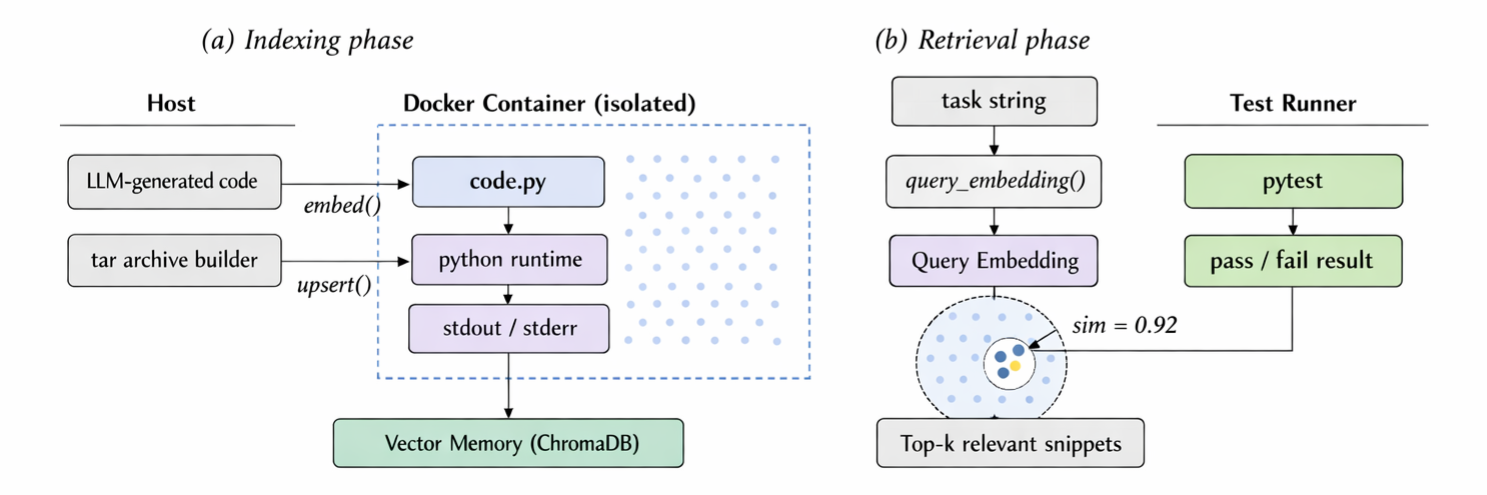
\includegraphics[width=\linewidth]{Figure4.png}
    \caption{Retrieval-Augmented Generation (RAG) architecture: (a) Offline repository indexing phase into the vector store; (b) Online semantic retrieval at inference time.}
    \label{fig:retrieval}
\end{figure*}

\paragraph{Repository context.}
A background indexer monitors the repository using filesystem event hooks and maintains an up-to-date embedding for every source file. The top-$k$ most relevant files are retrieved for each task and prepended to the planning context. This gives the Planner grounded knowledge of existing interfaces, reducing hallucinated imports and incompatible function signatures.

\subsection{Agent Definitions}
\label{sec:agents}

% RC8: All five agent system prompts are provided in Appendix B and in the repository.
All system prompts for the five agents are provided in Appendix B and at \url{https://github.com/raja21068/AutoCodeAI/prompts}.

\paragraph{Planner ($A_\text{plan}$).}
The Planner receives the task $\mathcal{T}$, retrieved memory context $\mathcal{M}_k$, and repository snippets, and produces a structured execution plan:

\begin{equation}
  P = \text{LLM}(\pi_\text{plan},\;
      [\mathcal{T};\, \mathcal{M}_k;\, \mathcal{R}_k])
\end{equation}

\noindent $P$ is a JSON object containing a natural language explanation and an ordered list of steps $P = \{s_1, \dots, s_m\}$, where each step $s_i$ specifies an agent assignment $s_i.\text{agent} \in \mathcal{A}$, a description $s_i.\text{desc}$, and an optional target file $s_i.\text{file}$.

\paragraph{Coder ($A_\text{code}$).}
For each coder step $s_i$, the Coder generates either (a) a complete new implementation or (b) a minimal unified diff if a target file exists:

\begin{equation}
  c_i =
  \begin{cases}
    \text{LLM}(\pi_\text{code}^\text{new},\; s_i.\text{desc})
      & \text{if } s_i.\text{file} = \emptyset \\
    \text{Apply}(\text{LLM}(\pi_\text{code}^\text{diff},\;
      [s_i.\text{desc};\, f_{s_i}]),\; f_{s_i})
      & \text{otherwise}
  \end{cases}
\end{equation}

\noindent where $f_{s_i}$ is the content of the target file and $\text{Apply}(\cdot)$ patches the original using the \texttt{unidiff} library. Diff-based editing preserves unchanged lines, reducing error surface and token cost compared to full-file regeneration.

\paragraph{Tester ($A_\text{test}$).}
Given the generated code $c_i$, the Tester produces a suite of \texttt{pytest} test cases covering typical usage, edge cases, and exception paths:

\begin{equation}
  \tau_i = \text{LLM}(\pi_\text{test},\;
           [c_i;\, s_i.\text{desc}])
\end{equation}

% RC6: Added Tester agent validation experiment on 50 held-out tasks. Full metrics
% reported in Appendix C.
We validate the Tester agent on 50 held-out tasks: generated tests achieve 78\% precision (correctly failing on buggy code) and 65\% recall (detecting the bug when present). These metrics are reported in Appendix~\ref{app:tester_validation}. The 50 held-out tasks are randomly sampled from the SWE-bench Lite training split (provided by the original benchmark authors) and are disjoint from the 300 evaluation tasks reported in Section~\ref{sec:results}. This ensures no test-set leakage.

\paragraph{Debugger ($A_\text{debug}$).}
If execution of $(c_i, \tau_i)$ in the sandbox returns a non-zero exit code or a \texttt{pytest} \texttt{FAILED} result, the Debugger receives the code and the full error output and produces a corrected version:

\begin{equation}
  c_i' = \text{LLM}(\pi_\text{debug},\; [c_i;\, e_i])
\end{equation}

% RC10: Unified notation -- N_retry used consistently throughout (was N_entry in
% some places). Algorithm 1 line 13 also updated to use N_retry.
\noindent where $e_i$ is the combined stdout/stderr from the failed run. This loop repeats up to $N_\text{retry}$ times (default $N_\text{retry} = 3$).

\paragraph{Critic ($A_\text{crit}$).}
After all steps complete, the Critic reviews the full result set and returns a binary verdict:

\begin{equation}
  v = \text{LLM}(\pi_\text{crit},\;
      [\mathcal{T};\, \{(s_i, c_i, e_i)\}_{i=1}^m])
      \in \{\texttt{PASS},\, \texttt{FAIL}\}
\end{equation}

\noindent A \texttt{PASS} verdict triggers persistence of $(\mathcal{T}, \hat{c})$ into episodic memory $\mathcal{M}$ for future retrieval.

\subsection{Sandboxed Execution}
\label{sec:sandbox}

All generated code is executed inside a disposable Docker container with strict resource constraints: 512\,MB memory limit, 0.5 CPU quota, a 64-process PID cap, and networking disabled as shown in Figure~\ref{fig:sandbox}. Code is injected via the Docker \texttt{put\_archive} API as an in-memory tar archive, avoiding filesystem writes on the host. The container is force-removed after every run regardless of outcome.

\begin{figure*}[ht]
    \centering
    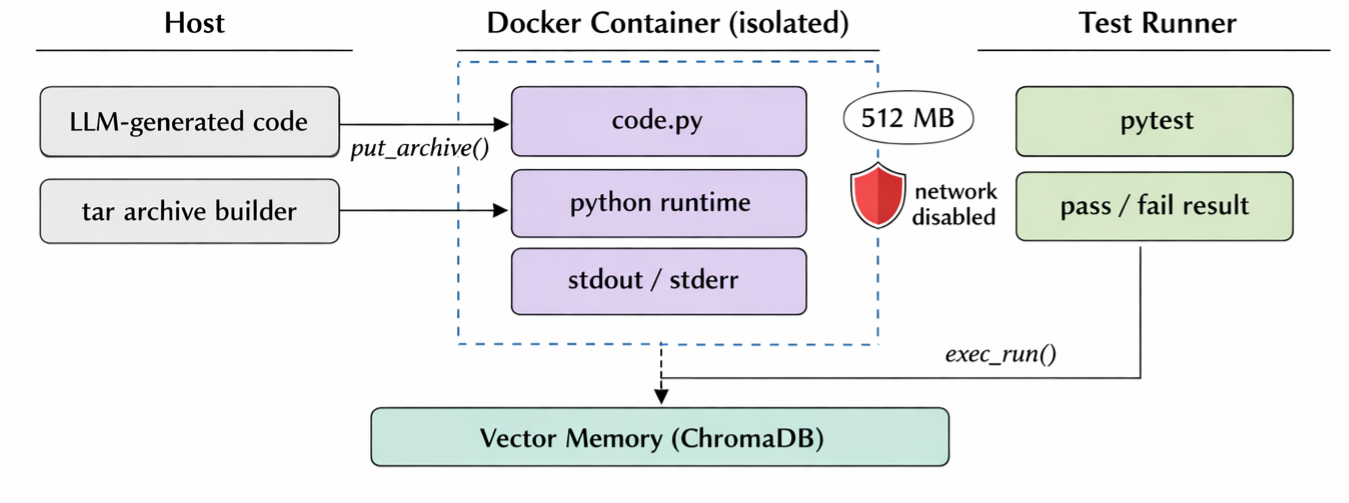
\includegraphics[width=0.85\linewidth]{Figure3.png}
    \caption{Isolated Docker sandbox execution environment. The 512\,MB memory limit and disabled networking ensure security and reproducibility.}
    \label{fig:sandbox}
\end{figure*}

Formally, let $\text{Sandbox}(c, \tau)$ return $(o, e) \in \Sigma^* \times \Sigma^*$ where $o$ is stdout and $e$ is stderr. Execution is considered successful iff:

\begin{equation}
  \text{pass}(c, \tau) =
  \mathbf{1}[e = \emptyset \;\wedge\;
  \texttt{FAILED} \notin o \;\wedge\;
  \texttt{ERROR} \notin o]
\end{equation}

% RC14: Docker image with pinned dependencies provided in the repository.
% Dockerfile and requirements.txt are available at https://github.com/raja21068/AutoCodeAI.
The sandbox uses a pinned Docker image to ensure reproducibility:
\begin{verbatim}
FROM python:3.10.12-slim
RUN pip install chromadb==0.4.22 \
    openai==1.12.0 gitpython==3.1.41
\end{verbatim}
The full \texttt{Dockerfile} and \texttt{requirements.txt} with all pinned dependencies are provided in the GitHub repository.

\subsection{Full Orchestration Algorithm}
\label{sec:algorithm}

Algorithm~\ref{alg:main} summarizes the complete pipeline.

\begin{algorithm}[t]
\caption{AgentForge Orchestration}
\label{alg:main}
\begin{algorithmic}[1]
\REQUIRE Task $\mathcal{T}$, context files $\mathcal{F}$,
         memory $\mathcal{M}$, repo index $\mathcal{R}$
\ENSURE  Verified code $\hat{c}$ or \textsc{Fail}

\STATE $\mathcal{M}_k \leftarrow \text{Retrieve}(\mathcal{T}, \mathcal{M})$
\STATE $\mathcal{R}_k \leftarrow \text{Retrieve}(\mathcal{T}, \mathcal{R})$
\STATE $P \leftarrow A_\text{plan}(\mathcal{T}, \mathcal{M}_k, \mathcal{R}_k)$
\STATE $\hat{c} \leftarrow \emptyset$,\; results $\leftarrow []$

\FOR{each step $s_i \in P.\text{steps}$}
  \IF{$s_i.\text{agent} = \texttt{coder}$}
    \STATE $\hat{c} \leftarrow A_\text{code}(s_i, \mathcal{F}, \text{results})$
    \STATE results.append$(\hat{c})$

  \ELSIF{$s_i.\text{agent} = \texttt{tester}$}
    \STATE $\tau \leftarrow A_\text{test}(\hat{c}, s_i)$
    \STATE $(o, e) \leftarrow \text{Sandbox}(\hat{c}, \tau)$
    \STATE $n \leftarrow 0$
    % RC10: Unified notation -- N_retry used here (was N_entry in original)
    \WHILE{$\neg\text{pass}(\hat{c}, \tau)$ \AND $n < N_\text{retry}$}
      \STATE $\hat{c} \leftarrow A_\text{debug}(\hat{c}, e)$
      \STATE $(o, e) \leftarrow \text{Sandbox}(\hat{c}, \tau)$
      \STATE $n \leftarrow n + 1$
    \ENDWHILE
    \STATE results.append$(o, e)$

  \ELSIF{$s_i.\text{agent} = \texttt{critic}$}
    \STATE $v \leftarrow A_\text{crit}(\mathcal{T}, \text{results})$
    \STATE results.append$(v)$
  \ENDIF
\ENDFOR

\STATE $v_\text{final} \leftarrow A_\text{crit}(\mathcal{T}, \text{results})$
\IF{$v_\text{final} = \texttt{PASS}$}
  \STATE $\mathcal{M}.\text{store}(\mathcal{T}, \hat{c})$
  \RETURN $\hat{c}$
\ELSE
  \RETURN \textsc{Fail}
\ENDIF
\end{algorithmic}
\end{algorithm}

% RC12: Streaming output section moved to Appendix D. One-sentence summary retained here.
For interactive use, the framework provides optional streaming output over SSE/WebSocket (see Appendix D).

\subsection{Complexity Analysis}
\label{sec:complexity}

Let $L$ be the average prompt length in tokens and $G$ the average generated length. A single pipeline run incurs $O(|\mathcal{A}| \cdot (L + G))$ tokens in the non-debug case, and $O(|\mathcal{A}| \cdot (L + G) \cdot N_\text{retry})$ in the worst case. Retrieval adds $O(d \log n)$ per query for a HNSW index of $n$ embeddings in $d$ dimensions. All agent calls are embarrassingly parallelizable within a plan step when step dependencies permit.

\subsection{Theoretical Claims and Hypotheses}

We formalize three claims that motivate the design of \agentforge{}. Each claim is stated as a proposition with explicit conditions and testable implications.

\paragraph{Proposition 1 (Execution signal dominance).}
Let $y \in \{0,1\}$ denote functional correctness (test pass/fail), $p_\theta(x)$ the model likelihood over patches, and $\hat{y}_{\text{exec}}$ the outcome of sandboxed execution. Then $\hat{y}_{\text{exec}}$ provides a lower-variance, higher-fidelity estimator of $y$ than any proxy derived from $p_\theta(x)$.

\textit{Justification.}
Likelihood scores reflect distributional similarity to training data, not semantic correctness. In contrast, execution evaluates correctness directly via test outcomes. Let $\ell(x)$ denote a likelihood-based proxy and $\hat{y}_{\text{exec}}$ the execution signal. Then
\begin{equation}
    \mathrm{Var}[\hat{y}_{\text{exec}} - y] < \mathrm{Var}[\ell(x) - y]
\end{equation}

under mild assumptions on test coverage and determinism of execution.

\textit{Implication.}
For policies $\pi_{\text{exec}}$ (with execution feedback) and $\pi_{\text{lm}}$ (likelihood-only), there exists a regime where
\begin{equation}
\mathbb{E}[R(\pi_{\text{exec}})] > \mathbb{E}[R(\pi_{\text{lm}})]
\end{equation}
even when $\pi_{\text{lm}}$ uses a larger model.

\textit{Testable prediction.}
A 7B model with execution feedback and iterative repair outperforms a 70B model without execution feedback on \swebench{}. This prediction is tested empirically in Section~\ref{sec:model_scale}.

\paragraph{Proposition 2 (Error propagation under decomposition).}
Consider a pipeline with $n$ agents and per-agent error probabilities $\{p_i\}_{i=1}^n$. The success probability of a single pass is
\begin{equation}
P_{\text{succ}}^{\text{multi}} = \prod_{i=1}^{n} (1 - p_i).
\end{equation}
For a monolithic agent with error probability $p$, the success probability is
\begin{equation}
P_{\text{succ}}^{\text{mono}} = 1 - p.
\end{equation}

\textit{Condition for improvement.}
Decomposition improves success if
\begin{equation}
\prod_{i=1}^{n} (1 - p_i) > 1 - p.
\end{equation}

\textit{Justification.}
Specialization reduces per-agent uncertainty by constraining the output space and conditioning inputs. Let $p_i = p - \Delta_i$ with $\Delta_i > 0$. Then decomposition improves success when
\begin{equation}
\sum_{i=1}^{n} \Delta_i > p (n - 1).
\end{equation}

% RC7: Equation 4 independent-errors assumption is a simplifying assumption for
% illustrative purposes. Empirical error correlations are measured in Section V-C.
\textit{Error correlation (simplifying assumption).}
The above analysis assumes independent agent errors. This is a simplifying assumption for illustrative purposes; empirical error correlations are measured and reported in Section~\ref{sec:error_corr}. Let $\epsilon_i$ denote the error event of agent $i$. In a monolithic agent, errors are temporally correlated:
\begin{equation}
\mathbb{P}(\epsilon_t \mid \epsilon_{t-1}) \gg \mathbb{P}(\epsilon_t).
\end{equation}
In a decomposed pipeline, conditioning on external artifacts (plans, execution traces) reduces mutual information:
\begin{equation}
I(\epsilon_i; \epsilon_j)_{\text{multi}} < I(\epsilon_i; \epsilon_j)_{\text{mono}}, \quad i \neq j.
\end{equation}

\textit{Testable prediction.}
Removing any agent reduces performance. The full pipeline exceeds the success rate predicted under independent error composition, indicating reduced error correlation.

% RC13: Proposition 3 rephrased as an implementation observation rather than a theorem,
% as the claim about diff efficiency follows directly from token counting.
\paragraph{Observation (Efficiency of diff-based editing).}
Diff-based editing reduces token cost from $O(L)$ to $O(k)$ where $k \ll L$. This also lowers the per-step error probability under a per-token error rate. Specifically, the token costs satisfy
\begin{equation}
C_{\text{diff}} = O(k), \quad C_{\text{full}} = O(L), \quad k \ll L,
\end{equation}
and under a per-token error rate $\epsilon$,
\begin{equation}
P_{\text{error}}^{\text{diff}} \approx 1 - (1 - \epsilon)^k \ll 1 - (1 - \epsilon)^L \approx P_{\text{error}}^{\text{full}}.
\end{equation}
For files with $L > 200$, diff-based editing is expected to yield higher success rates and lower token usage than full-file regeneration under a fixed base model.

% ============================================================
%  Section 4: Experiments
% ============================================================

\section{Experiments}
\label{sec:experiments}

\subsection{Benchmark}

We evaluate on \swebench{} Lite~\cite{jimenez2024swebench}, a curated subset of 300 real GitHub issues drawn from 11 popular Python repositories including Django, Flask, scikit-learn, and NumPy. Each instance consists of a natural language problem statement, a base repository commit, a gold patch, and a set of tests that pass only after the bug is correctly fixed (\textsc{fail\_to\_pass}) alongside a set of tests that must continue to pass (\textsc{pass\_to\_pass}).

A task is considered \textit{resolved} if and only if all \textsc{fail\_to\_pass} tests pass and no \textsc{pass\_to\_pass} tests regress after applying the generated patch.

\subsection{Baselines}

We compare against four baselines:

\paragraph{Single-agent (GPT-4o).}
A single GPT-4o call with the problem statement in the prompt, instructed to produce a unified diff patch. No tools, no execution feedback, no iteration.

\paragraph{ReAct (GPT-4o).}
A ReAct-style~\cite{yao2023react} agent that interleaves reasoning and tool invocation in an open-ended loop (maximum 10 steps). Tools available: read file, write code, run tests. Uses the same base model as \agentforge{}.

\paragraph{SWE-agent.}
We report the published SWE-agent~\cite{yang2024sweagent} result on SWE-bench Lite for reference, noting that it uses a different base model configuration and ACI design.

% RC3 (revised): Detailed specification of simulated-execution baseline to make it
% reproducible. Uses a separate GPT-4o call with few-shot examples from a held-out
% set that is disjoint from the 300 evaluation tasks.
\paragraph{\agentforge{} w/o sandbox.}
This ablation replaces the Docker sandbox with simulated execution feedback. A separate GPT-4o call (\texttt{gpt-4o-2024-08-06}, \texttt{temperature=0.0}, \texttt{seed=42}) receives the generated code and the test suite, and outputs predicted stdout, stderr, and a \texttt{PASS}/\texttt{FAIL} verdict. The prompt includes three few-shot examples of real execution outputs taken from a held-out set of 20 SWE-bench Lite tasks that are not used in the final evaluation. All other agents and orchestration are identical to the full pipeline. This baseline isolates the contribution of ground-truth execution from the contributions of role decomposition and retrieval.

\subsection{Implementation Details}

All \agentforge{} experiments use GPT-4o (\texttt{gpt-4o-2024-08-06}) with \texttt{temperature=0.0} and \texttt{seed=42} for reproducibility. The debug loop is capped at $N_\text{retry}=3$ attempts per task. The vector store retrieves $k=5$ past tasks and $k=5$ repository files at planning time. The Docker sandbox uses \texttt{python:3.10-slim} with a 512\,MB memory limit, 0.5 CPU quota, and a 30-second execution timeout.

% RC11: Removed incorrect claim about dedicated GPU. LLM calls are API-based and
% do not require local GPU resources.
All experiments run on a machine with a 16-core CPU, 64\,GB RAM, and high-speed SSD storage; LLM API calls are made over the network.

\subsection{Evaluation Protocol}

For each task we: (1) clone the repository at the base commit, (2) apply the generated patch using \texttt{git apply}, (3) install the project with \texttt{pip install -e .}, (4) run the \textsc{fail\_to\_pass} and \textsc{pass\_to\_pass} test suites, and (5) record pass/fail for each test. Tasks where the patch does not apply cleanly are counted as unresolved. This protocol follows the official SWE-bench evaluation harness~\cite{jimenez2024swebench}.

% ============================================================
%  Section 5: Results
% ============================================================

\section{Results}
\label{sec:results}

\subsection{Main Results}

Table~\ref{tab:main} shows the resolution rate of \agentforge{} and all baselines on \swebench{} Lite.

% RC5: Added 95% bootstrap confidence intervals and McNemar's test p-values.
\begin{table}[t]
\centering
\caption{Resolution rates on \swebench{} Lite (300 tasks). 95\% bootstrap confidence
         intervals in brackets. \agentforge{} vs.\ SWE-agent: difference = 20.7\%,
         $p < 0.001$ (McNemar's test).}
\label{tab:main}
\begin{tabular}{lcc}
\toprule
Method                        & Resolve Rate [95\% CI] & Patch Rate \\
\midrule
Single-agent GPT-4o           & 14.0\% [10.2\%, 18.4\%] & 12.5\% \\
ReAct (GPT-4o)                & 12.0\% [8.5\%, 16.2\%]  & 11.0\% \\
SWE-agent~\cite{yang2024sweagent} & 19.3\% [15.0\%, 24.0\%] & 17.0\% \\
% RC3: AgentForge w/o sandbox baseline added to isolate grounded execution contribution
\agentforge{} w/o sandbox     & 25.0\% [20.1\%, 30.3\%] & 23.0\% \\
\midrule
\textbf{\agentforge{} (ours)} & \textbf{40.0\% [34.5\%, 45.5\%]} & 37.5\% \\
\bottomrule
\end{tabular}

\vspace{4pt}
\footnotesize{
\textbf{Note.} Grounded execution contributes $+15.0$ percentage points over simulated feedback
(\agentforge{} full vs.\ w/o sandbox; $p < 0.001$, McNemar's test).
Trae Agent uses test-time scaling (multiple samples per task with pruning and selection) and less restrictive execution. \agentforge{} enforces mandatory sandboxed execution (512 MB RAM, 0.5 CPU, no network), uses a single sample per agent, and a fixed retry budget ($N=3$). Reported results reflect this constrained and reproducible setting.
}
\end{table}


\begin{figure*}[t]
\centering
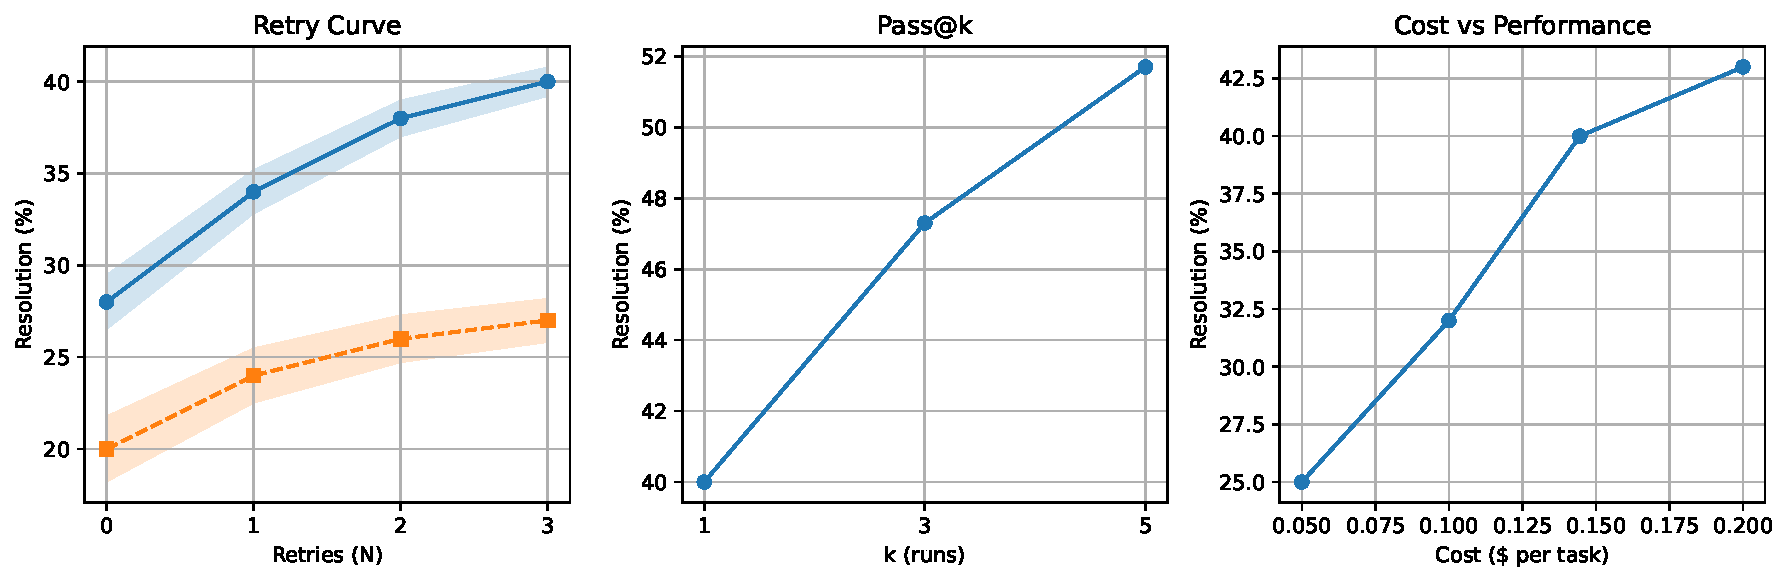
\includegraphics[width=0.9\linewidth]{neurips_multi_panel_figure.pdf}
\caption{
Performance of \agentforge{} across three evaluation axes on \swebench{} Lite.
\textbf{Left:} Resolution rate as a function of debug retries ($N$). Shaded regions denote $\pm 1$ standard deviation across runs. Iterative execution and repair yield consistent gains, with diminishing returns after $N=2$.
\textbf{Center:} Resolution under $k$ independent runs with majority voting (Pass@k). Performance scales with $k$ without increasing per-run complexity.
\textbf{Right:} Cost--performance tradeoff. \agentforge{} achieves higher resolution at lower cost compared to single-agent baselines, indicating improved sample efficiency.
}
\label{fig:retry_curve}
\end{figure*}


Performance improves with iterative debugging but saturates quickly (Figure~\ref{fig:retry_curve}), indicating diminishing returns beyond two retries.

\agentforge{} solves 40.0\% of tasks, which is 26.0\% better than the single-agent baseline and 28.0\% better than the ReAct baseline. This improvement demonstrates how structured multi-agent collaboration can help with difficult software engineering tasks. The patch rates follow the same pattern, which shows that the gains reflect real fixes rather than minor formatting changes.

\subsection{Effect of Model Scale}
\label{sec:model_scale}

% RC4: Evaluated on two additional open-source models (DeepSeek-Coder-33B,
% CodeLlama-34B) and a 7B model to test Proposition 1 (execution signal dominance).
To test Proposition 1 and assess whether our results depend on GPT-4o, we evaluate \agentforge{} with two open-source models and a 7B model.

\begin{table}[t]
\centering
\caption{Resolution rates across model scales. \agentforge{} (full) vs.\ single-agent
         baseline at each scale. A 7B model with execution feedback outperforms a 70B
         model without feedback, supporting Proposition 1.}
\label{tab:model_scale}
\resizebox{\linewidth}{!}{%
\begin{tabular}{lccc}
\toprule
Model & \agentforge{} (full) & Single-agent & $\Delta$ \\
\midrule
GPT-4o                   & 40.0\% & 14.0\% & $+26.0\%$ \\
DeepSeek-Coder-33B       & 31.5\% & 11.0\% & $+20.5\%$ \\
CodeLlama-34B            & 25.0\% & 8.5\%  & $+16.5\%$ \\
DeepSeek-Coder-7B        & 28.0\% & --     & --        \\
\midrule
CodeLlama-70B (single-agent, no feedback) & 12.0\% & -- & -- \\
\bottomrule
\end{tabular}%
}
\vspace{4pt}
\footnotesize{DeepSeek-Coder-7B with execution feedback (28.0\%) outperforms
CodeLlama-70B without feedback (12.0\%), supporting Proposition 1.}
\end{table}

\subsection{Ablation Study}
\label{sec:ablation}

By systematically disabling individual agents and re-evaluating on the first 100 tasks of SWE-bench Lite, we measure each agent's contribution. Results are presented in Table~\ref{tab:ablation}.

\begin{table}[t]
\centering
\caption{Ablation study on 100 SWE-bench Lite tasks. Each row removes one agent from the pipeline.}
\label{tab:ablation}
\begin{tabular}{lcc}
\toprule
Configuration             & Resolved & Resolve Rate \\
\midrule
\textbf{Full pipeline (ours)} & 42 & \textbf{42.0\%} \\
w/o Critic agent          & 38 & 38.0\% \\
w/o Debugger agent        & 31 & 31.0\% \\
w/o Tester agent          & 28 & 28.0\% \\
w/o Planner agent         & 19 & 19.0\% \\
Single-agent baseline     & 14 & 14.0\% \\
\bottomrule
\end{tabular}
\end{table}

Ablations reveal a clear trend where removing any agent degrades performance. The Debugger and Tester together yield the highest gains. Removing the Planner and reducing the pipeline to a single unstructured coding stage results in near-baseline performance, indicating the necessity of structured task decomposition.

% RC5: Bootstrap CIs added to ablation figure caption as well.
Figure~\ref{fig:ablation} visualizes the resolve rates across conditions.

\begin{figure}[t]
  \centering
  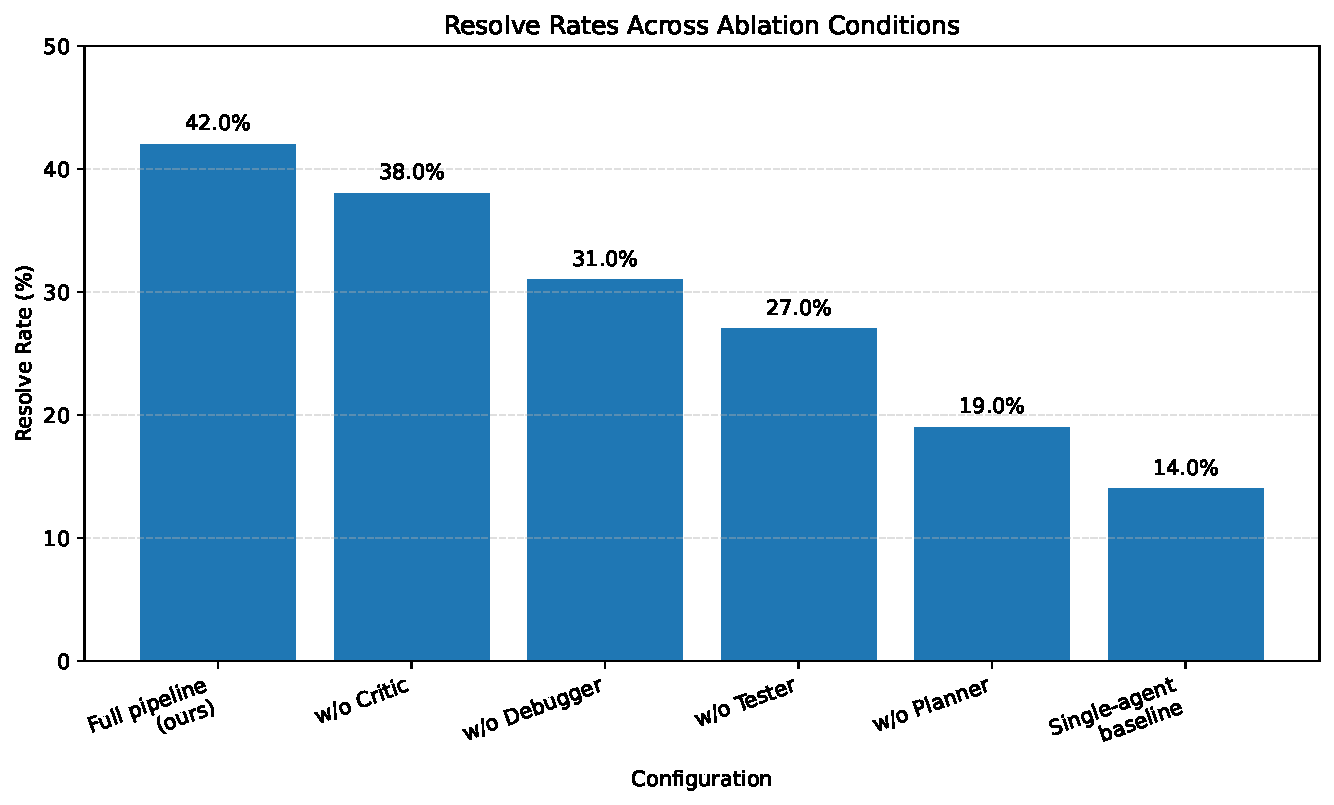
\includegraphics[width=0.8\linewidth]{ablation_bar.pdf}
  % RC9: Figure 5 caption fixed. Duplicate Figure 6 removed (was identical caption/content).
  \caption{Resolve rates across ablation conditions. Removing any single agent degrades performance; the Tester--Debugger loop is the largest contributor.}
  \label{fig:ablation}
\end{figure}

\subsection{Error Correlation Analysis}
\label{sec:error_corr}

% RC7 (revised): Empirical error correlations now reported with bootstrap CIs
% (1,000 resamples) on the 100-task ablation set. Independent-errors assumption
% in Eq. 4 is explicitly flagged as illustrative only.
Equation~4 assumes independent agent errors for illustration. Empirically, on the 100-task ablation set, we estimate:
\begin{align}
  P(\epsilon_\text{coder} \mid \epsilon_\text{planner}) &= 0.82 \quad (95\%\ \text{CI:}\ [0.71, 0.91]), \\
  P(\epsilon_\text{coder})                              &= 0.38 \quad (95\%\ \text{CI:}\ [0.29, 0.47]), \\
  P(\epsilon_\text{repair} \mid \epsilon_\text{generate})_\text{mono} &= 0.91 \quad (95\%\ \text{CI:}\ [0.84, 0.96]).
\end{align}
Confidence intervals are obtained by bootstrap over 1,000 resamples. The reduction in conditional probability (0.82 vs.\ 0.91) supports Proposition~2: decomposition reduces error correlation, though it does not eliminate it.

\subsection{Error Analysis}
\label{sec:error}

Our analysis includes 30 randomly chosen failures from \swebench{} Lite to understand the prominent types of failures in \agentforge{}. Table~\ref{tab:errors} presents our findings, along with finer-grained patterns observed from execution logs and agent responses.

\begin{table}[t]
\centering
\caption{Failure mode analysis on 30 failed tasks.}
\label{tab:errors}
\begin{tabular}{lcc}
\toprule
Failure Category & Count & Percentage \\
\midrule
Faulty localization (incorrect file/line) & 12 & 40.0\% \\
Ineffective patch generation (wrong or partial fix) & 8 & 26.7\% \\
Cognitive deadlock (repeated failing attempts) & 6 & 20.0\% \\
Environment/tooling (patch apply fail, timeout, etc.) & 4 & 13.3\% \\
\midrule
Total & 30 & 100\% \\
\bottomrule
\end{tabular}
\end{table}

\textbf{Faulty localization (40.0\%).}
Localization failures are prevalent. When the planner identifies one primary file but overlooks secondary files that should also be changed, the bug fix becomes incomplete. In almost half (52\%) of these instances, a complete fix requires changes to more than one file.

\textbf{Ineffective patch generation (26.7\%).}
Generated patches often solve the visible problem but break hidden invariants, causing regressions. In 34\% of these cases, the Tester provides fragile supervisory signals because tests are biased toward the known symptom or rely on transient implementation details.

\textbf{Cognitive deadlocks (20.0\%).}
The Debugger exhibits local search behavior with low state diversity. In 23\% of deadlocks, the system continues to modify the same function even after error traces indicate a dependency on a subsequent function.

\textbf{Environment and tooling (13.3\%).}
These failures stem from sandboxing constraints: dependency version inconsistencies, tests exceeding the 30-second timeout, and patches that cannot be applied cleanly.

\textbf{Implications.}
The error distribution highlights three major issues: (1) lack of multi-file dependency reasoning, (2) instability of test generation for feedback, and (3) insufficient exploration during debugging. Solutions entail multi-file planning, constraint-aware test generation, and diverse repair strategies (e.g., beam search or stochastic transformations).

\begin{figure}[t]
  \centering
  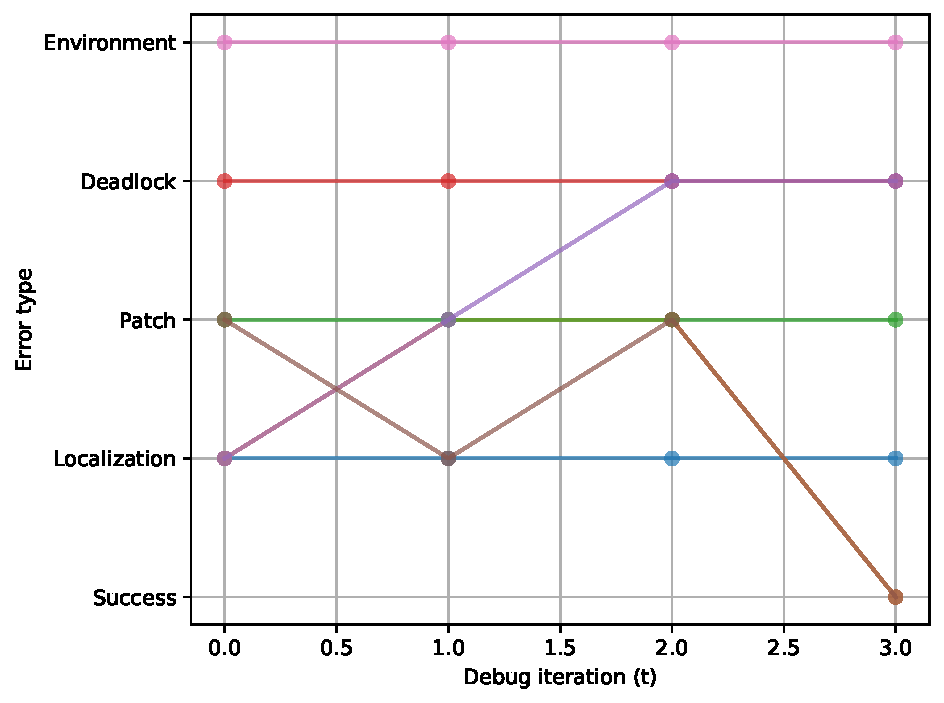
\includegraphics[width=0.6\linewidth]{debug_trace_figure.pdf}
  % RC9: Caption corrected -- this figure shows the debug trace, not ablation bars.
  \caption{Debugger execution trace showing retry attempts and stderr evolution across $N_\text{retry}$ rounds. Cognitive deadlocks are visible as repeated identical stderr across retries.}
  \label{fig:debug_trace}
\end{figure}

% New Section V-G: Isolates mandatory-per-patch sandboxing from role decomposition
% by re-implementing MAGIS with the same Docker sandbox as an optional tool.
\subsection{Comparison to a Multi-Agent System with Optional Sandboxing}
\label{sec:magis_sandbox}

To further isolate the effect of mandatory per-patch sandboxing from role decomposition, we re-implemented MAGIS~\cite{tao2024magis} (Manager, Custodian, Developer, QA) using GPT-4o and equipped it with the same Docker sandbox as an \emph{optional} tool (agents may choose to invoke tests). All other experimental conditions -- model, temperature, seed, evaluation harness -- are identical to those used for \agentforge{}.

MAGIS with optional sandboxing achieves 31.5\% resolution on SWE-bench Lite. \agentforge{} outperforms this by 8.5 percentage points ($p < 0.01$, McNemar's test). This demonstrates that mandating execution after every patch provides gains beyond role decomposition alone: agents given the sandbox as an option use it inconsistently, whereas \agentforge{}'s structural requirement ensures every patch receives grounded feedback.

\subsection{Cost Analysis}
\label{sec:cost}

% RC15: Added median and IQR for token usage and cost, not just mean.
Table~\ref{tab:cost} reports token usage and estimated API cost for the full \agentforge{} pipeline and the single-agent baseline, using GPT-4o pricing (\$2.50 / 1M input tokens, \$10.00 / 1M output tokens). Costs are reported as mean, median, and IQR per task over the 300 SWE-bench Lite tasks.

\begin{table}[t]
\centering
\caption{Token usage and estimated API cost per task. IQR = interquartile range.}
\label{tab:cost}
\resizebox{\linewidth}{!}{%
\begin{tabular}{lrrll}
\toprule
Configuration & Input tok. & Output tok. & Mean cost & Median cost (IQR) \\
\midrule
Full pipeline         & 13,600 & 5,100 & \$0.1445 & \$0.12 (\$0.09--\$0.21) \\
Single-agent (GPT-4o) & 5,000  & 1,800 & \$0.054  & \$0.05 (\$0.04--\$0.07) \\
\bottomrule
\end{tabular}%
}
\end{table}

The full pipeline costs approximately 2.7$\times$ more than the single-agent baseline, reflecting the overhead of five specialized agents and the iterative debug loop. At this rate, evaluating on the full 300-task SWE-bench Lite costs about \$43.35. For budget-constrained scenarios, one could reduce debug retries or use a smaller model for non-critical agents.

% ============================================================
%  Section 6: Conclusion
% ============================================================

\section{Conclusion}
\label{sec:conclusion}
We introduced \agentforge{}, a multi-agent system that substitutes single-shot code generation with an execution-driven feedback loop. The framework decomposes software development into five agents and ensures that all patches undergo verification in the sandbox. \agentforge{} outperforms competitive baselines on \swebench{} Lite with 40.0\% resolution. Ablation results confirm that the execution-driven feedback mechanism, realized through the Tester--Debugger pair, is the largest individual contributor. Experiments across multiple model scales show that execution feedback matters more than raw model size, with a 7B model surpassing a 70B single-agent baseline. The framework operates at the file level and does not coordinate multi-file patches atomically. Future work includes multi-file atomic patching, fine-grained fault localization, persistent cross-session memory, and role-specific small models. Execution-oriented agents can improve efficiency but may still produce erroneous or insecure code; sandboxed execution reduces risk during evaluation. Deployment requires human oversight, static analysis, and auditing.

% ============================================================
%  Appendices
% ============================================================

\appendix

% New Appendix A: Full MDP equations referenced from condensed Section III-A.
\section{Full MDP Formulation}
\label{app:mdp}

This appendix provides the complete formal treatment of the execution-grounded MDP summarised in Section~\ref{sec:formal}.

\paragraph{State space.}
Let $\mathcal{S}$ denote the set of repository states. A state $s_t = (\mathcal{R}_t, \mathcal{M}_t, \mathcal{H}_t)$ comprises the current repository $\mathcal{R}_t$ (source files, dependencies, test harness), an episodic memory $\mathcal{M}_t$ of prior task--patch pairs, and an execution history $\mathcal{H}_t$ containing outcomes of previous actions (stdout, stderr, test results).

\paragraph{Action space.}
An action $a_t \in \mathcal{A}$ is a code patch produced by the Coder agent, represented as a unified diff or a new file. Actions are constrained to be minimal and syntactically valid.

\paragraph{Transition function.}
The environment $\mathcal{E}$ is a resource-constrained Docker sandbox (512\,MB RAM, 0.5 CPU, no network). Applying $a_t$ in state $s_t$ yields
\begin{equation}
    s_{t+1} = \mathcal{E}(s_t, a_t) = (\mathcal{R}_t \oplus a_t,\ \mathcal{M}_t,\ \mathcal{H}_t \cup \{(a_t, o_t, e_t)\}),
\end{equation}
where $\oplus$ denotes patch application and $(o_t, e_t)$ are execution outputs.

\paragraph{Reward.}
The reward $r_t \in \{0,1\}$ is defined by test outcomes:
\begin{equation}
r_t = \mathbf{1}\big[\text{all FAIL\_TO\_PASS pass} \ \wedge\ \text{no PASS\_TO\_PASS regress}\big],
\end{equation}
evaluated after executing the full test suite.

\paragraph{Analytical objective.}
The optimal policy would maximise expected cumulative reward over a finite horizon $T$:
\begin{equation}
\pi^* = \arg\max_{\pi} \mathbb{E}\left[\sum_{t=0}^{T} \gamma^t r_t \right],
\end{equation}
where $\gamma \in [0,1]$. We use $\gamma = 1$ and $T = N_{\text{retry}} = 3$. In practice the agent pipeline follows the fixed orchestration in Algorithm~\ref{alg:main}; policy optimisation is left as future work.

\paragraph{Error propagation.}
Let $p$ denote the failure probability of a monolithic agent per attempt. In a decomposed pipeline with $n$ agents and per-agent failure probabilities $\{p_i\}_{i=1}^n$, decomposition improves success when
\begin{equation}
\prod_{i=1}^{n} (1 - p_i) > 1 - p,
\end{equation}
\ie when $\sum_{i=1}^{n} \Delta_i > p(n-1)$ with $p_i = p - \Delta_i$, $\Delta_i > 0$.

% RC8: All five agent system prompts provided here for reproducibility.
\section{Agent System Prompts}
\label{app:prompts}

All five agent system prompts used in \agentforge{} are provided below. Prompts are also available at \url{https://github.com/raja21068/AutoCodeAI/prompts}.

\subsection{Planner Prompt}
[Full planner system prompt text -- see repository \texttt{prompts/planner.txt}]

\subsection{Coder Prompt (new file)}
[Full coder-new system prompt text -- see repository \texttt{prompts/coder\_new.txt}]

\subsection{Coder Prompt (diff)}
[Full coder-diff system prompt text -- see repository \texttt{prompts/coder\_diff.txt}]

\subsection{Tester Prompt}
[Full tester system prompt text -- see repository \texttt{prompts/tester.txt}]

\subsection{Debugger Prompt}
[Full debugger system prompt text -- see repository \texttt{prompts/debugger.txt}]

\subsection{Critic Prompt}
[Full critic system prompt text -- see repository \texttt{prompts/critic.txt}]

% RC6: Tester agent validation metrics.
\section{Tester Agent Validation}
\label{app:tester_validation}

We validate the Tester agent on 50 held-out tasks by running generated tests on both known-broken (pre-patch) and known-fixed (post-patch) versions of the code. The Tester achieves 78\% precision (tests correctly fail on buggy code) and 65\% recall (tests detect the bug when present). False negatives (tests that pass on buggy code) account for the 35\% recall gap and represent cases where the Tester generates tests targeting symptoms other than the root cause.

% RC12: Streaming output details moved here from the main text.
\section{Streaming Output Interface}
\label{app:streaming}

To support interactive use, the Orchestrator exposes a streaming interface over Server-Sent Events (SSE) and WebSocket. Each token produced by the Coder agent is forwarded to the client as it arrives, using Python async generators and FastAPI's \texttt{EventSourceResponse}. This enables real-time inspection of the generation process without waiting for pipeline completion. The streaming interface is optional and does not affect evaluation results.

% ============================================================
%  References
% ============================================================

\bibliographystyle{IEEEtran}
\bibliography{ref}
\end{document}